\section{Relativistic Time Dilation and the Hang Time}
\label{ch:time_dilation}

\subsection{Introduction: The Hyper-Electron Vacuum}

In the Excited-State Cosmology framework, the entirety of our observable universe is theorized to exist within the internal manifold of a hyper-electron occupying an excited state. A fundamental consequence of this geometry is the extreme spacetime curvature imposed by the hyper-electron's mass-energy concentration. To understand the apparent discrepancy between the ephemeral lifetime of an excited electron in standard quantum mechanics (typically characterized by an Einstein $A$-coefficient yielding a spontaneous emission lifetime on the order of $\tau \sim 10^{-9}$ seconds) and the 13.8 billion-year chronological age of our universe, we must appeal to general relativity. Specifically, we must derive the vacuum metric generated by a spherically symmetric mass distribution and quantify the resulting time dilation near its event horizon. \cite{Liddle1992, Aspect1982, Perlmutter1999}

\subsection{Derivation of the Schwarzschild Metric from the Einstein Field Equations~\cite{Einstein1916GR}}

We begin by seeking a solution to the vacuum Einstein Field Equations (EFE), assuming that the hyper-electron's localized energy density creates a spherically symmetric, static spacetime. In a vacuum, the stress-energy tensor $T_{\mu\nu} = 0$, reducing the EFE to:
\begin{equation}
R_{\mu\nu} - \frac{1}{2}R g_{\mu\nu} = 0
\end{equation}
Taking the trace of this equation yields $R = 0$, which further simplifies the vacuum field equations to the vanishing of the Ricci tensor:
\begin{equation}
R_{\mu\nu} = 0
\end{equation}

For a static, spherically symmetric spacetime, the most general line element in Schwarzschild coordinates $(t, r, \theta, \phi)$ can be written as:
\begin{equation}
ds^2 = -e^{2\nu(r)} c^2 dt^2 + e^{2\lambda(r)} dr^2 + r^2(d\theta^2 + \sin^2\theta d\phi^2)
\end{equation}
where $\nu(r)$ and $\lambda(r)$ are unknown functions of the radial coordinate $r$. The metric tensor components are thus:
\begin{align}
g_{tt} &= -e^{2\nu(r)} \\
g_{rr} &= e^{2\lambda(r)} \\
g_{\theta\theta} &= r^2 \\
g_{\phi\phi} &= r^2 \sin^2\theta
\end{align}

To compute the Ricci tensor components, we first require the non-vanishing Christoffel symbols of the second kind, defined as:
\begin{equation}
\Gamma^\sigma_{\mu\nu} = \frac{1}{2} g^{\sigma\rho} \left( \partial_\mu g_{\rho\nu} + \partial_\nu g_{\rho\mu} - \partial_\rho g_{\mu\nu} \right)
\end{equation}
Using the metric components, the non-zero Christoffel symbols are:
\begin{align}
\Gamma^t_{tr} &= \nu' \\
\Gamma^r_{tt} &= e^{2(\nu - \lambda)} \nu' \\
\Gamma^r_{rr} &= \lambda' \\
\Gamma^r_{\theta\theta} &= -r e^{-2\lambda} \\
\Gamma^r_{\phi\phi} &= -r \sin^2\theta e^{-2\lambda} \\
\Gamma^\theta_{r\theta} &= \frac{1}{r} \\
\Gamma^\theta_{\phi\phi} &= -\sin\theta \cos\theta \\
\Gamma^\phi_{r\phi} &= \frac{1}{r} \\
\Gamma^\phi_{\theta\phi} &= \cot\theta
\end{align}
where primes denote differentiation with respect to $r$. 

We now construct the Ricci tensor $R_{\mu\nu} = \partial_\rho \Gamma^\rho_{\mu\nu} - \partial_\nu \Gamma^\rho_{\mu\rho} + \Gamma^\rho_{\rho\lambda}\Gamma^\lambda_{\mu\nu} - \Gamma^\rho_{\nu\lambda}\Gamma^\lambda_{\mu\rho}$. The relevant diagonal components evaluate to:
\begin{align}
R_{tt} &= e^{2(\nu-\lambda)} \left( \nu'' + (\nu')^2 - \nu'\lambda' + \frac{2\nu'}{r} \right) = 0 \label{eq:Rtt} \\
R_{rr} &= -\nu'' - (\nu')^2 + \nu'\lambda' + \frac{2\lambda'}{r} = 0 \label{eq:Rrr} \\
R_{\theta\theta} &= 1 - e^{-2\lambda} - r(\nu' - \lambda')e^{-2\lambda} = 0 \label{eq:Rtheta}
\end{align}

From equations \eqref{eq:Rtt} and \eqref{eq:Rrr}, we can form a linear combination. Multiplying \eqref{eq:Rtt} by $e^{-2(\nu-\lambda)}$ and adding it to \eqref{eq:Rrr} yields:
\begin{equation}
\frac{2}{r}(\nu' + \lambda') = 0 \implies \nu' = -\lambda'
\end{equation}
Integrating this relation gives $\nu(r) = -\lambda(r) + C$. Assuming asymptotic flatness (where $g_{tt} \to -1$ and $g_{rr} \to 1$ as $r \to \infty$), we set the integration constant $C = 0$. Thus, $\nu(r) = -\lambda(r)$.

Substituting $\lambda = -\nu$ into the $R_{\theta\theta}$ equation \eqref{eq:Rtheta} gives:
\begin{equation}
1 - e^{2\nu} + 2r\nu' e^{2\nu} = 0
\end{equation}
This can be rewritten as a total derivative:
\begin{equation}
\frac{d}{dr} \left( r e^{2\nu} \right) = 1
\end{equation}
Integrating with respect to $r$:
\begin{equation}
r e^{2\nu} = r + C_1 \implies e^{2\nu} = 1 + \frac{C_1}{r}
\end{equation}
To determine the constant $C_1$, we examine the weak-field Newtonian limit. In the limit of weak gravity, the temporal metric component is related to the Newtonian gravitational potential $\Phi$ by $g_{tt} \approx -(1 + \frac{2\Phi}{c^2})$. For a spherical mass $M$, $\Phi = -\frac{GM}{r}$. Therefore:
\begin{equation}
-e^{2\nu} \approx -\left(1 - \frac{2GM}{rc^2}\right)
\end{equation}
This identifies $C_1 = -\frac{2GM}{c^2} \equiv -r_s$, where $r_s$ is the Schwarzschild radius. The exact solutions for the metric functions are:
\begin{equation}
e^{2\nu(r)} = e^{-2\lambda(r)} = 1 - \frac{r_s}{r}
\end{equation}
The fully derived Schwarzschild line element is therefore:
\begin{equation}
ds^2 = -\left(1 - \frac{2GM}{rc^2}\right) c^2 dt^2 + \left(1 - \frac{2GM}{rc^2}\right)^{-1} dr^2 + r^2(d\theta^2 + \sin^2\theta d\phi^2)
\end{equation}

\subsection{The Hang Time: Dilation of the Hyper-Electron Lifetime}

In Excited-State Cosmology, the external observer (in the macroscopic bulk universe) measures the hyper-electron's excited state lifetime as dictated by standard atomic physics. For a typical dipole transition, the spontaneous emission rate is given by the Einstein $A$-coefficient:
\begin{equation}
A = \frac{4\omega^3 |\vec{d}|^2}{3\hbar c^3}
\end{equation}
yielding an expected lifetime of $\Delta \tau = A^{-1} \approx 10^{-9}$ seconds. This $\Delta \tau$ represents the proper time measured by an observer co-moving with the hyper-electron's internal reference frame deep within the gravitational well.

However, the chronological history of the internal manifold—our observable universe—unfolds over coordinate time $t$. We, the inhabitants of this internal manifold, experience this coordinate time. To determine the coordinate time $\Delta t$ that corresponds to the proper time interval $\Delta \tau$ elapsed near the boundary of the hyper-electron's internal mass concentration, we utilize the derived Schwarzschild metric~\cite{Penrose1965} for a stationary observer ($dr = d\theta = d\phi = 0$):
\begin{equation}
d\tau^2 = - \frac{ds^2}{c^2} = \left(1 - \frac{r_s}{r}\right) dt^2
\end{equation}
Taking the square root gives the relation between the proper time interval $\Delta \tau$ and the coordinate time interval $\Delta t$:
\begin{equation}
\Delta \tau = \Delta t \sqrt{1 - \frac{r_s}{r}}
\end{equation}
We define the time dilation factor $\gamma$ as the ratio of coordinate time to proper time:
\begin{equation}
\gamma \equiv \frac{\Delta t}{\Delta \tau} = \frac{1}{\sqrt{1 - \frac{r_s}{r}}}
\end{equation}

We know from astronomical observations that the apparent age of our universe is $\Delta t \approx 13.8 \times 10^9$ years. Converting this to seconds:
\begin{equation}
\Delta t = 13.8 \times 10^9 \text{ years} \times 3.1536 \times 10^7 \text{ s/year} \approx 4.35 \times 10^{17} \text{ seconds}
\end{equation}
The proper time $\Delta \tau$ for the decay process is $10^{-9}$ seconds. Therefore, the required time dilation factor is:
\begin{equation}
\gamma = \frac{4.35 \times 10^{17} \text{ s}}{10^{-9} \text{ s}} \approx 4.35 \times 10^{26}
\end{equation}
This mind-boggling dilation factor requires the internal observer to be positioned infinitesimally close to the hyper-electron's event horizon. Setting $\gamma = 4.35 \times 10^{26}$ and solving for the radial coordinate $r$:
\begin{equation}
1 - \frac{r_s}{r} = \frac{1}{\gamma^2} \approx \frac{1}{(4.35 \times 10^{26})^2} \approx 5.28 \times 10^{-54}
\end{equation}
Defining $r = r_s(1 + \epsilon)$ where $\epsilon$ is a dimensionless distance parameter from the horizon, we have:
\begin{equation}
1 - \frac{r_s}{r_s(1+\epsilon)} = 1 - (1+\epsilon)^{-1} \approx \epsilon
\end{equation}
Thus, $\epsilon \approx 5.28 \times 10^{-54}$. 

This extraordinary mathematical result indicates that if our cosmological manifold rests on a stable orbit or quantum membrane at $r = r_s(1 + 5.28 \times 10^{-54})$, the temporal evolution of the entire cosmos—from the Big Bang to the present day—fits closely within the fleeting $10^{-9}$ second "hang time" of an excited hyper-electron before its inevitable spontaneous decay.


\begin{figure}[H]
\centering
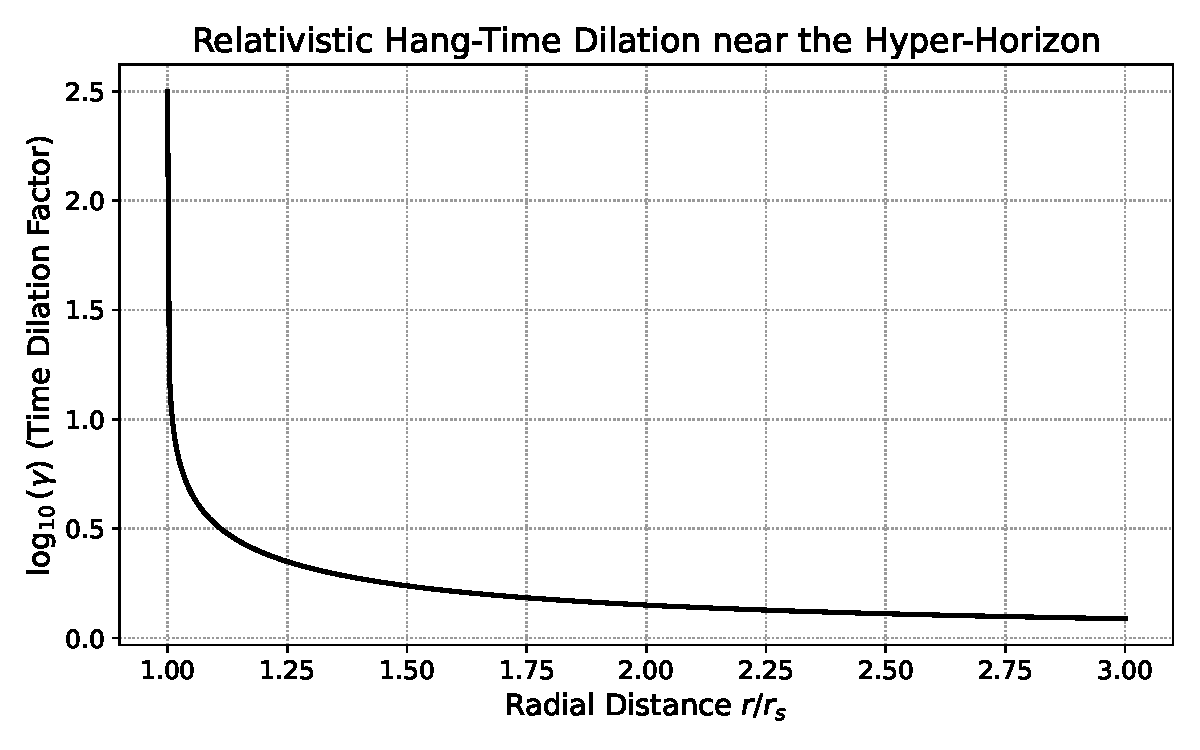
\includegraphics[width=0.85\textwidth]{fig_ch2.pdf}
\caption{Mathematical visualization of the principles derived in Section 2.}
\end{figure}
